\documentclass{beamer}

\mode<presentation>
{
    \usetheme{Warsaw}
}

\title{CycleMLP}
\subtitle{A MLP-like Architecture for Dense Prediction}
\author{Marco Benelli}
\institute{University of Florence}
\date{February 14, 2022}

\begin{document}

\begin{frame}
    \titlepage
\end{frame}

\begin{frame}{Outline}
    \tableofcontents
\end{frame}

\section{Introduction}

\begin{frame}{Paradigm shifts}
    Recent paradigm shifts:
    \begin{description}
        \item[2012] AlexNet
        \item[2020] ViT
        \item[2021] MLP-Mixer
    \end{description}
\end{frame}

\begin{frame}{MLP-Mixer}
    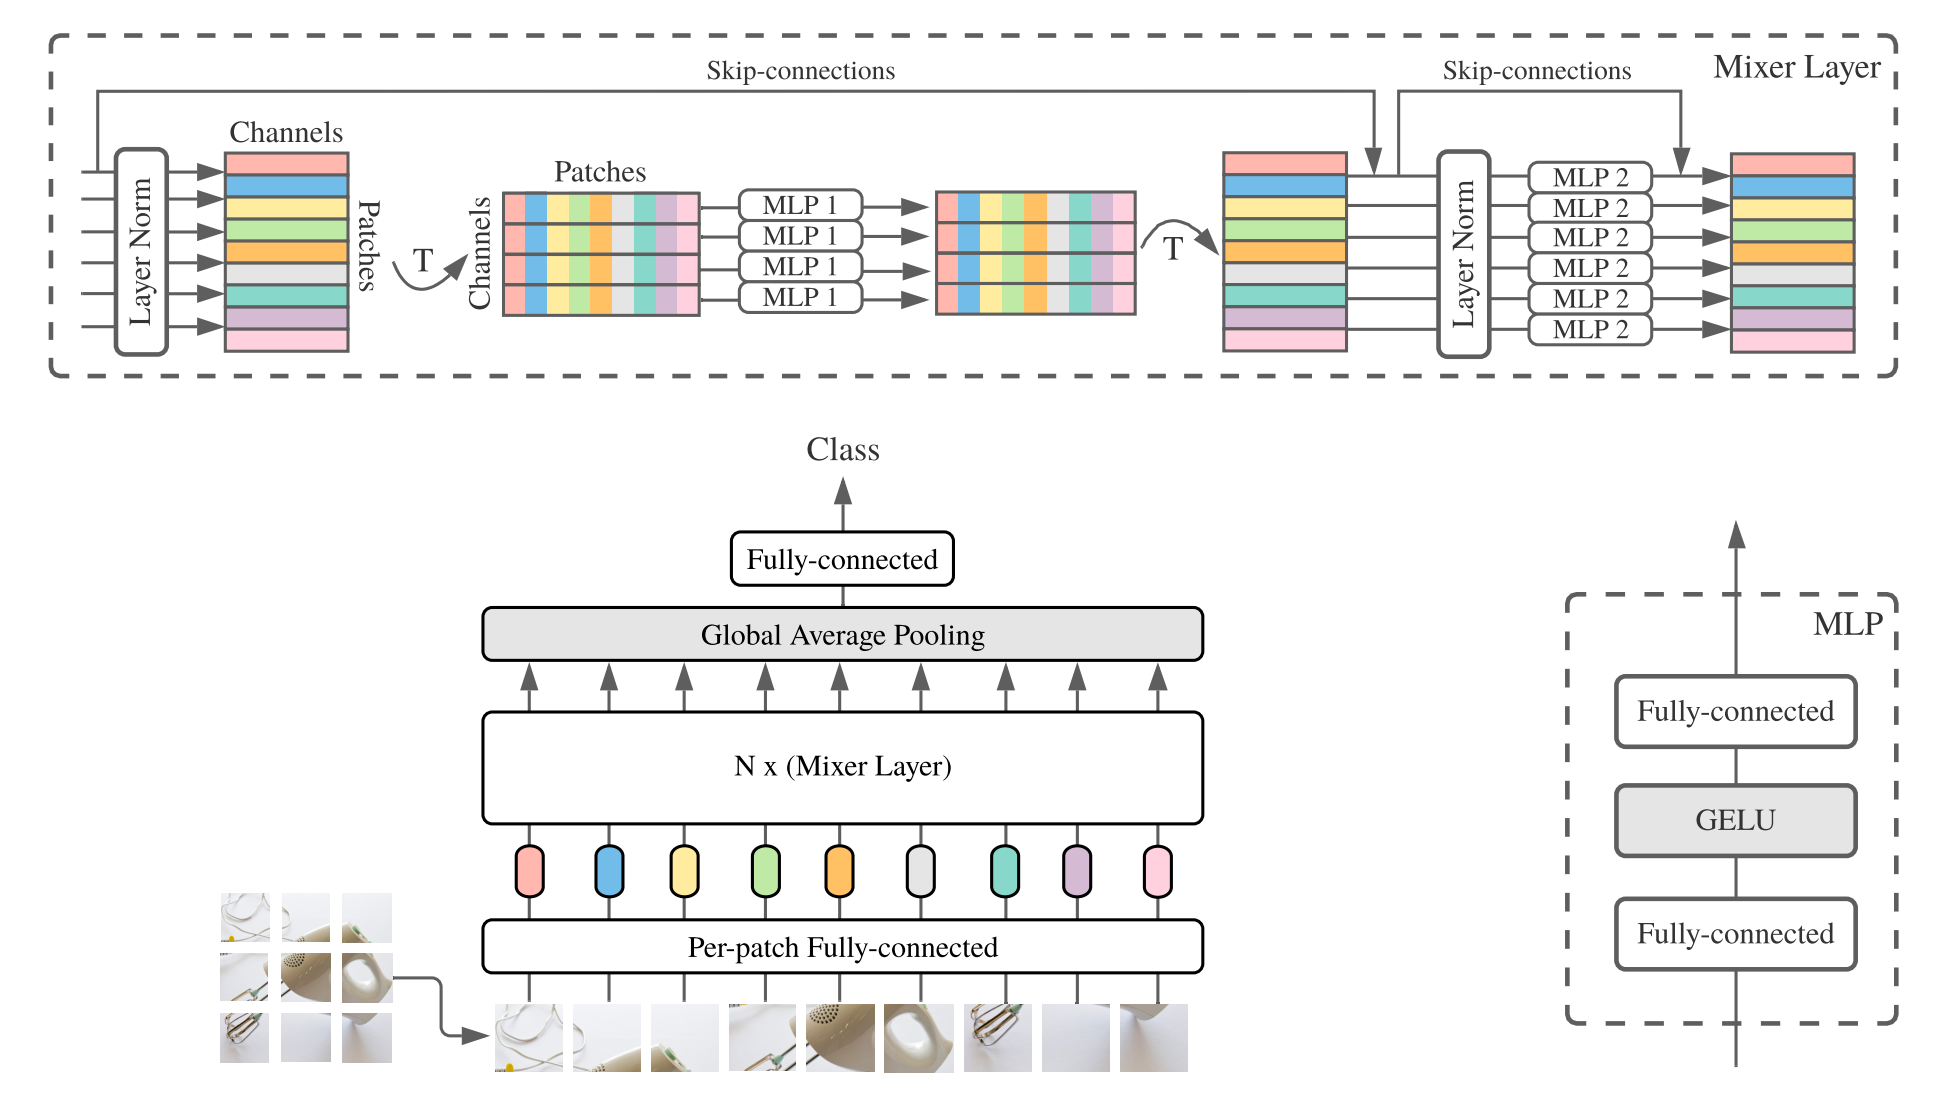
\includegraphics[width=\textwidth]{figures/mixer_figure.png}
\end{frame}

\begin{frame}{Challenges}
    MLP-like models are facing these challenges:
    \begin{itemize}
        \item non-hierarchical architectures
        \item flexible input scales
        \item quadratic costs
    \end{itemize}
\end{frame}

\begin{frame}{MLP-Mixer v. CycleMLP}
    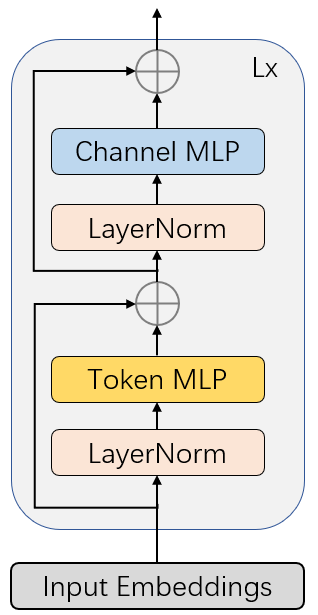
\includegraphics[width=.4\textwidth]{figures/mlp_mixer.png}
    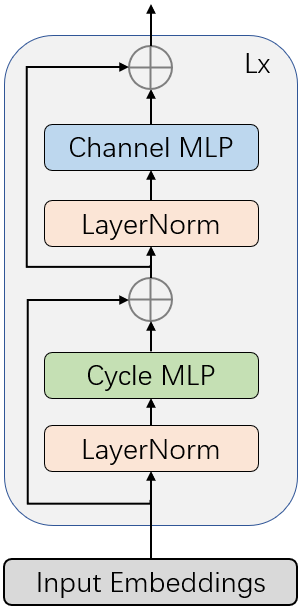
\includegraphics[width=.4\textwidth]{figures/cycle_mlp.png}
\end{frame}

\section{Method}

\subsection{Cycle Fully-Connected Layer}
\subsection{Overall Architecture}

\section{Experiments}

\subsection{STL10 Classification}

\begin{frame}
    % table
\end{frame}

\section{Conclusion}

\section*{Summary}

\begin{frame}{Summary}
    \begin{itemize}
    \item The \alert{first main message} of your talk in one or two lines.
    \item The \alert{second main message} of your talk in one or two lines.
    \item Perhaps a \alert{third message}, but not more than that.
    \end{itemize}
\end{frame}

\end{document}
